%% Copernicus Publications Manuscript Preparation Template for LaTeX Submissions
%% ---------------------------------
%% This template should be used for copernicus.cls
%% The class file and some style files are bundled in the Copernicus Latex Package which can be downloaded from the different journal webpages.
%% For further assistance please contact the Copernicus Publications at: publications@copernicus.org
%% http://publications.copernicus.org


%% Please use the following documentclass and Journal Abbreviations for Discussion Papers and Final Revised Papers.


%% 2-Column Papers and Discussion Papers
\documentclass[esd, manuscript]{copernicus}



%% Journal Abbreviations (Please use the same for Discussion Papers and Final Revised Papers)

% Archives Animal Breeding (aab)
% Atmospheric Chemistry and Physics (acp)
% Advances in Geosciences (adgeo)
% Advances in Statistical Climatology, Meteorology and Oceanography (ascmo)
% Annales Geophysicae (angeo)
% ASTRA Proceedings (ap)
% Atmospheric Measurement Techniques (amt)
% Advances in Radio Science (ars)
% Advances in Science and Research (asr)
% Biogeosciences (bg)
% Climate of the Past (cp)
% Drinking Water Engineering and Science (dwes)
% Earth System Dynamics (esd)
% Earth Surface Dynamics (esurf)
% Earth System Science Data (essd)
% Fossil Record (fr)
% Geographica Helvetica (gh)
% Geoscientific Instrumentation, Methods and Data Systems (gi)
% Geoscientific Model Development (gmd)
% Geothermal Energy Science (gtes)
% Hydrology and Earth System Sciences (hess)
% History of Geo- and Space Sciences (hgss)
% Journal of Sensors and Sensor Systems (jsss)
% Mechanical Sciences (ms)
% Natural Hazards and Earth System Sciences (nhess)
% Nonlinear Processes in Geophysics (npg)
% Ocean Science (os)
% Proceedings of the International Association of Hydrological Sciences (piahs)
% Primate Biology (pb)
% Scientific Drilling (sd)
% SOIL (soil)
% Solid Earth (se)
% The Cryosphere (tc)
% Web Ecology (we)
% Wind Energy Science (wes)


%% \usepackage commands included in the copernicus.cls:
%\usepackage[german, english]{babel}
%\usepackage{tabularx}
%\usepackage{cancel}
%\usepackage{multirow}
%\usepackage{supertabular}
%\usepackage{algorithmic}
%\usepackage{algorithm}
%\usepackage{amsthm}
%\usepackage{float}
%\usepackage{subfig}
%\usepackage{rotating}


\begin{document}

\title{TEXT}


% \Author[affil]{given_name}{surname}

\Author[1]{Doug}{McNeall}
\Author[2]{Jonny}{Williams}
\Author[1]{Ben}{Booth}
\Author[1]{Richard}{Betts}
\Author[3]{Peter}{Challenor}
\Author[1]{Andrew}{Wiltshire}
\Author[1]{David}{Sexton}


\affil[1]{Met Office Hadley Centre, FitzRoy Road, Exeter, EX1 3PB UK}
\affil[2]{NIWA, New Zealand}
\affil[3]{University of Exeter, North Park Road, Exeter EX4 4QE UK}

%% The [] brackets identify the author with the corresponding affiliation. 1, 2, 3, etc. should be inserted.



\runningtitle{TEXT}

\runningauthor{TEXT}

\correspondence{Doug McNeall (doug.mcneall@metoffice.gov.uk)}



\received{}
\pubdiscuss{} %% only important for two-stage journals
\revised{}
\accepted{}
\published{}

%% These dates will be inserted by Copernicus Publications during the typesetting process.


\firstpage{1}

\maketitle



\begin{abstract}
We use observations of forest fraction to constrain carbon cycle and land surface input parameters of the reduced resolution global climate model, FAMOUS. Using a history matching approach along with a computationally cheap statistical proxy (emulator) of the climate model, we compare an ensemble of simulations of forest fraction with observations, and rule out parameter settings where the forests are poorly simulated. 

Regions of parameter space where FAMOUS best simulates the Amazon forest fraction are incompatible with the regions where FAMOUS best simulates other forests. Previous studies using climate models have used similar methods to find previously untried candidate input parameter sets that remove what was assumed an underlying structural error. We offer a counter example, arguing that we have found a true structural discrepancy. This has implications for the calibration of FAMOUS: using observations of different forest regions to calibrate the model leads to very different conclusions about the best values, the corresponding uncertainty of input parameters, and potentially, predictions of future forest cover. Dealing with this structural discrepancy is vital when choosing a set of "best" parameters for the land surface - failure to do so could lead to poor parameter selection.

We characterise the structural model discrepancy, and explore the consequences of ignoring it in a history matching exercise. We perform a sensitivity analysis to find the parameters most responsible for simulator error and therefore most promising for tuning.  We use the emulator to simulate the forest fraction at the best set of parameters implied by matching the model to the Amazon, and to other major forests in turn. We can find parameters that lead to a realistic forest fraction in the Amazon, but using the Amazon alone to tune the simulator would result in a significant overestimate of forest fraction in the other forests. Conversely, using the other forests to calibrate the model leads to a larger underestimate of the Amazon forest fraction.

Finally, we perform a history matching exercise using credible estimates for simulator discrepancy and observational uncertainty terms. We find that we are unable to constrain the parameters individually, but that just under half of joint parameter space is ruled out as being incompatible with forest observations. We discuss the possible sources of the discrepancy in the simulated Amazon, including missing processes in the land surface component, and a bias in the climatology of the Amazon.
\end{abstract}


\introduction  %% \introduction[modified heading if necessary]
 
A common practice in Earth system modelling is the parameterisation of processes which are too computationally expensive to represent explicitly. These parameterisations have associated numerical coefficients, quantitatively representing some process. The coefficients may directly represent a measurable physical quantity, or they may be a more abstract representation necessary due to the simplification of the modelled process. There is often uncertainty about the value of the any parameter coefficient that should be used to best represent the system being simulated. It may not be desirable or practical to choose a single value of the coefficients over all others, and uncertainty in the best choice of parameters can be represented by using a range of values for each of the coefficients in an ensemble of simulator runs. 

Choosing appropriate values of these coefficients is a major research effort that encompasses domain specific, statistical and computational literature. The coefficients are tuneable by comparison of the behaviour of the simulator with observations of the real system, although there may also be direct measurements of the value of the coefficient or other information from theory. There is a long history of using observations to constrain parameterisation coefficients within General Circulation Models (GCMs), particularly within atmospheric components. Where this is done as an inverse problem in formal probabilistic setting, then it may also provide probability distributions for the parameters of the model, and is known as \emph{calibration}. The process of choosing a single best parameter set is often called \emph{tuning}. \emph{History matching} provides a formal way of ruling out parameter settings that are inconsistent with observed data. 

The motivation for calibration of a simulator is twofold. First, a simulator which matches the underlying dynamics of a system well will produce more accurate predictions. Second, a more tightly constrained parameter set will provide a narrower range of uncertainty in future predictions. 

\subsection{Calibration of Land surface components}

Parametric uncertainty in the land surface and carbon cycle component of models is expected to represent a large fraction of current uncertainty in future climate projections (\citep{booth2012highsensitivity}, \citep{booth2013scenario}, \citep{huntingford2009contributions}). These components have been introduced into climate models more recently, and have not yet been subject to the depth of systematic evaluation as, for example, atmospheric components. There is much focus therefore, in identifying parameter sets that are consistent with observed climate metrics, or at least reducing future land carbon cycle uncertainty by identifying which parts of possible model parameter space are inconsistent with observed properties of the real climate system.  

There is also a long history of statistical and data assimilation approaches used to constrain process model parameters. In the land surface model context these extend back to \citep{sellers1996revised}. Recent examples are community efforts to develop a systematic set of observations to benchmark land surface processes against metrics of real world processes, for example the International Land Model Benchmarking Project \citep{luo2012framework}, and PALS \citep{abramowitz2012benchmarking}.  Such benchmarks involve an extensive set of metrics, covering a broad cross-section of model processes.  These benchmarks enable an assessment of overall model skill and highlight particular areas where the model falls short.  They provide a useful framework to assess improvements in model skill that arise from continual model development as well as prioritising resources towards model processes that are less well simulated.  The large number of observed metrics for diverse aspects of the model processes also help avoid model parameters being tuned to address a particular process, to the detriment of wider model performance. One of the limitations of the benchmarking approach is that there is only limited current understanding of what information a given observed metric implies about the model formulation or parameters, or what this might imply about future projected changes.


\subsection{Simulator discrepancy}

Simulator discrepancy is the systematic difference between a climate model, or simulator, and the system that is represented by that model. It can be known as model (or simulator) bias, model error, or structural error. A useful definition from \citep{williamson2014identifying} is that \emph{A climate model bias [simulator discrepancy] represents a structural error if that bias cannot be removed by changing the parameters without introducing more serious biases to the model}. One of the main aims of the model development process is to efficiently identify important simulator discrepancies and correct them, or allow them to be taken into account in analyses; for example, during prediction using the simulator.

Simulator discrepancy is a major challenge during calibration. In many cases, there is an indeterminacy between parameter error and simulator discrepancy; that is, should we choose a different set of parameters as representing the "best" or should we add a simulator discrepancy term? Sometimes, there is little or no information to distinguish between these two.

Simulator discrepancy might be known a priori - perhaps a computationally necessary simplification or parameterisation, has a predictable effect on simulator output. Alternatively, the discrepancy might be due to some missing and unknown process in the model. This sort of discrepancy might appear as a bias, and only become apparent when output from the simulator is compared with observations of the phenomena under study in the real system. In both cases, the modeller must have a strategy for dealing with the discrepancy when using the simulator to make judgements about the system.

\citep{kennedy2001bayesian} introduced a Bayesian framework to the task of the calibration of computationally expensive simulators. They urge the specification of a priori estimates of simulator discrepancy, and offer methods to learn about that discrepancy by comparison of the simulator and observations. Failure to take model discrepancy into account in calibration can lead to overconfident and inaccurate estimates of the parameters, and consequently the predictions of the model (e.g. \citep{brynjarsdottir2014learning}, \citep{higdon2008calibration}). Further, even inadequate (as opposed to outright wrong) specification of a simulator discrepancy can lead to overconfidence and bias in parameters and predictions.

\subsection{Paper aims and outline}

Our aim is to identify parameter sets for the land surface module of the climate simulator FAMOUS where the simulator output and the observations of forest fraction are consistent to an acceptable degree.  An initial attempt using history matching suggests that FAMOUS is unable to simulate the Amazon forest and other forests simultaneously at any set of parameters within the experiment design. We argue that this is due to a fundamental simulator discrepancy, which has implications for constraining the input parameters of FAMOUS. We use a number of techniques to characterise and find the drivers of this structural discrepancy, before performing a second history match with an appropriate discrepancy function.

In section \ref{sec:methods} we briefly describe the ensemble of a climate simulator, an emulator and the history matching technique that we use to explore simulator discrepancy. We perform an initial history matching exercise in section \ref{ssec:initial_history_match}. We use the emulator to quantify the relationships between the simulated forest fraction and a set of model input parameters in a sensitivity analysis in section \ref{sec:sensitivity}. Next, we measure the performance of the model ensemble in simulating forest fraction in section \ref{sec:confront}. We see how much input space would be ruled out as implausible in various scenarios of data combination and uncertainty budget in \ref{sec:combination} and we learn what each individual observation tells us about input space in section \ref{sec:learn}. In section \ref{sec:project}, we use the emulator and an implausibility measure to find the “best” set of parameters for each forest, and project the consequences of using those parameters on the other forests. Finally, we perform a history matching exercise with a credible discrepancy function in section \ref{sec:discrepancy}. In section \ref{sec:discussion}, we discuss the consequences of our findings for models of the Amazon rainforest. We offer conclusions in section \ref{sec:conclusions}.


\citep{craig1997pressure} 
\citep{booth2012highsensitivity}
\citep{booth2013scenario}
\citep{huntingford2009contributions} 
\citep{sellers1996revised}
\citep{abramowitz2012benchmarking}
\citep{luo2012framework}
\citep{williamson2014identifying}
\citep{kennedy2001bayesian}
\citep{brynjarsdottir2014learning}
\citep{higdon2008calibration}
\citep{jones2005systematic}
\citep{smith2008famous}
\citep{gordon2000simulation}
\citep{pope2000impact}
\citep{cox2001description}
\citep{smith2012famous}
\citep{williams2013optimising}
\citep{williams2014oxygen}
\citep{gnanadesikan2006diagnosing}
\citep{mckay1979comparison}
\citep{urban2010comparison}
\citep{gregoire2010optimal}
\citep{loveland2000landcover}
\citep{roustant2012dicekriging}
\citep{Rcore2016}
\citep{vernon2010galaxy}
\citep{lee2016aerosol}
\citep{williamson2013history}
\citep{ritz2015potential}
\citep{mcneall2013potential}
\citep{pukelsheim1994three}
\citep{carslaw2013large}
\citep{saltelli1999sensitivity}
\citep{Rpackage2015sensitivity}
\citep{cox2004amazon}
\citep{good2008objective}
\citep{joetzjer2013amazon}
\citep{staver2011determinants}
\citep{malhi2009amazon}
\citep{yin2012precipitation}



\section{HEADING}
TEXT

\subsection{HEADING}
TEXT

\subsubsection{HEADING}
TEXT

\conclusions  %% \conclusions[modified heading if necessary]
TEXT




\appendix
\section{}    %% Appendix A

\subsection{}                               %% Appendix A1, A2, etc.


\authorcontribution{TEXT}

\begin{acknowledgements}
TEXT
\end{acknowledgements}


%% REFERENCES

%% The reference list is compiled as follows:

%\begin{thebibliography}{}

%\bibitem[McNeall(2013)]{mcneall2013}
%REFERENCE 1

%\bibitem[AUTHOR(YEAR)]{LABEL}
%REFERENCE 2

%\end{thebibliography}

%% Since the Copernicus LaTeX package includes the BibTeX style file copernicus.bst,
%% authors experienced with BibTeX only have to include the following two lines:
%%
\bibliographystyle{copernicus}
\bibliography{famous.bib}
%%
%% URLs and DOIs can be entered in your BibTeX file as:
%%
%% URL = {http://www.xyz.org/~jones/idx_g.htm}
%% DOI = {10.5194/xyz}


%% LITERATURE CITATIONS
%%
%% command                        & example result
%% \citet{jones90}|               & Jones et al. (1990)
%% \citep{jones90}|               & (Jones et al., 1990)
%% \citep{jones90,jones93}|       & (Jones et al., 1990, 1993)
%% \citep[p.~32]{jones90}|        & (Jones et al., 1990, p.~32)
%% \citep[e.g.,][]{jones90}|      & (e.g., Jones et al., 1990)
%% \citep[e.g.,][p.~32]{jones90}| & (e.g., Jones et al., 1990, p.~32)
%% \citeauthor{jones90}|          & Jones et al.
%% \citeyear{jones90}|            & 1990



%% FIGURES

%f
\begin{figure}[t]
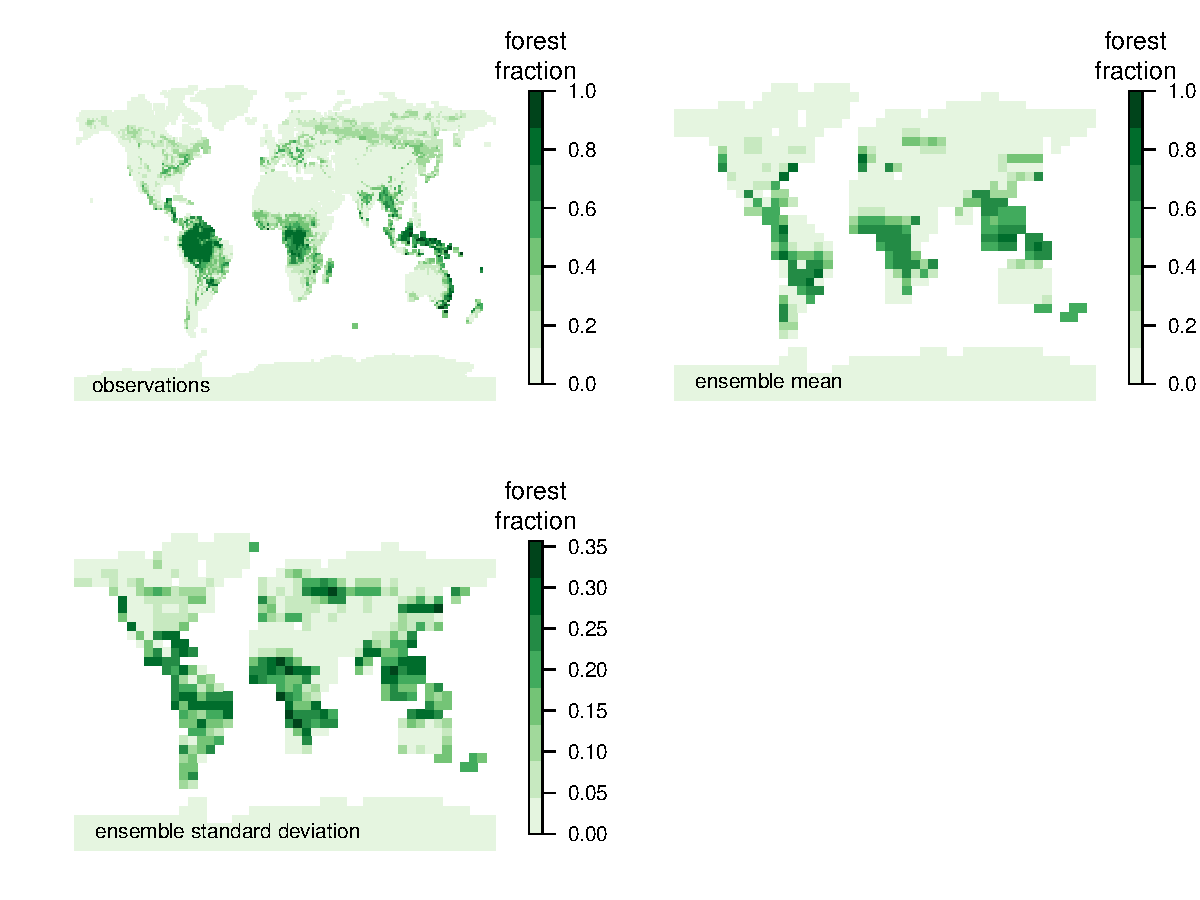
\includegraphics[width=12cm]{graphics/BL_obs_ensemble_mean_sd.pdf}
\caption{TEXT}
\label{fig:BL_obs_ensemble_mean_sd}
\end{figure}

\begin{figure}[t]
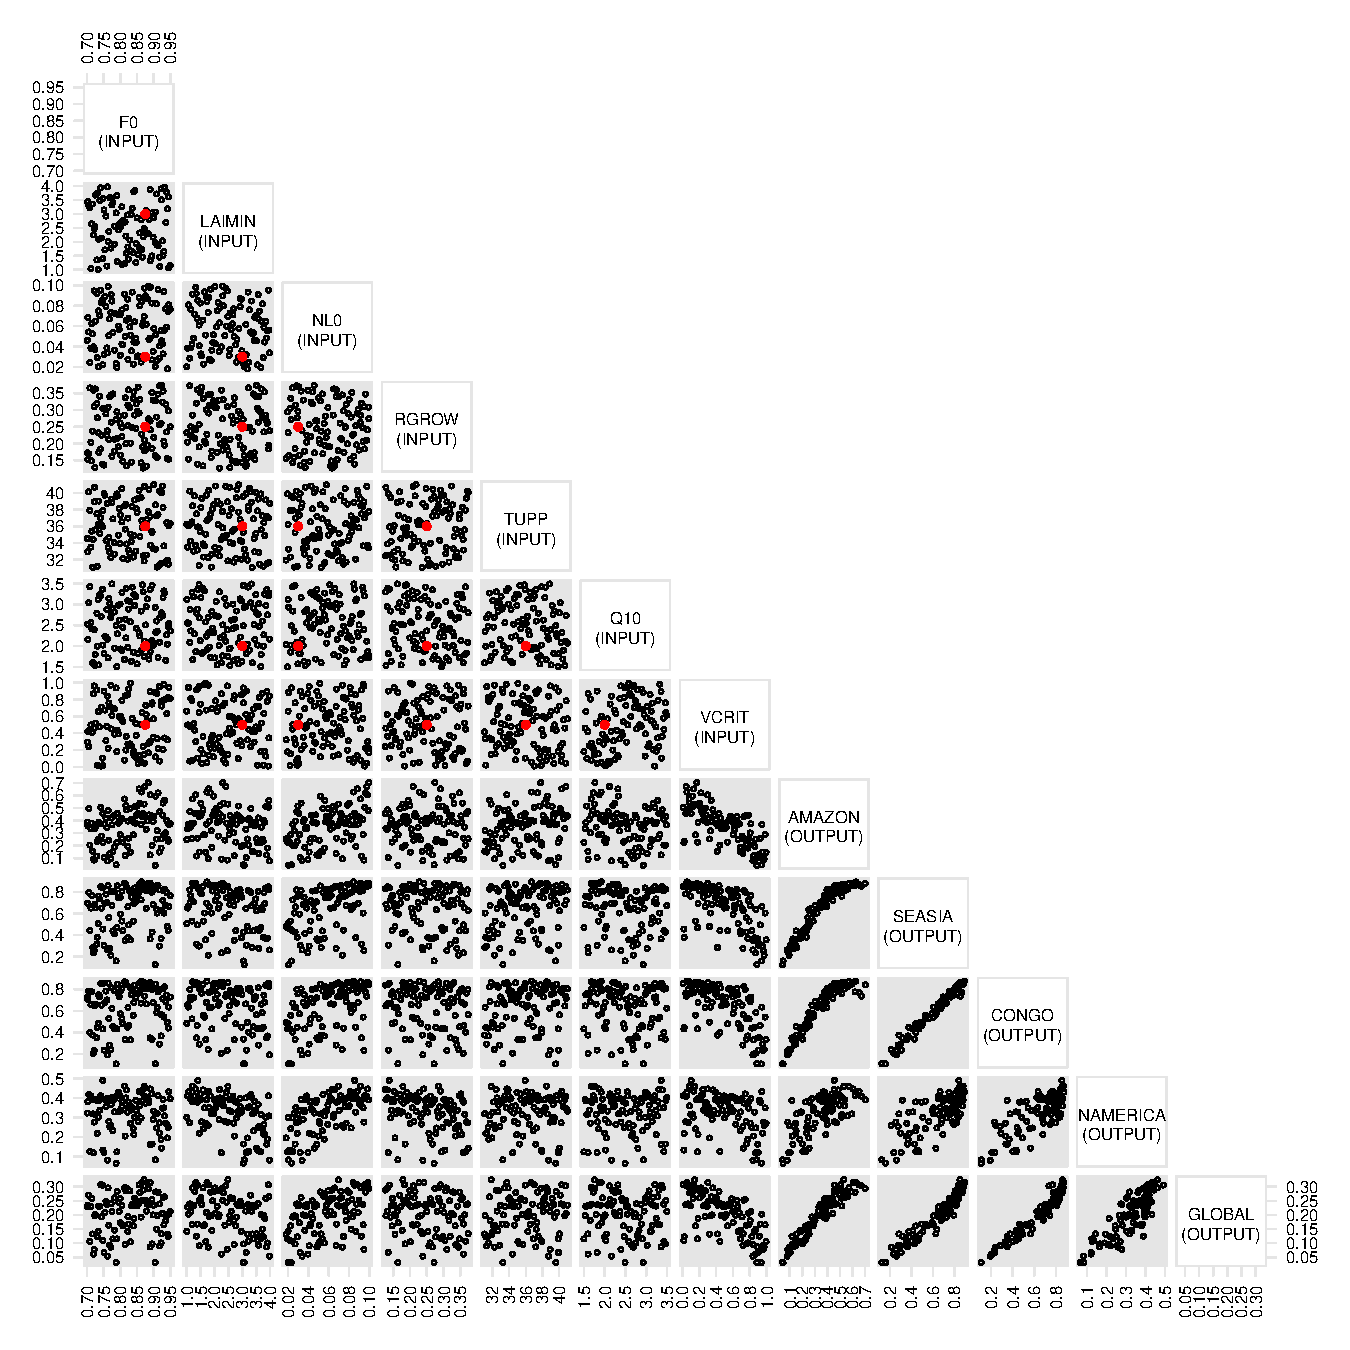
\includegraphics[width=12cm]{graphics/frac_pairs.pdf}
\caption{TEXT}
\label{fig:frac_pairs}
\end{figure}

\begin{figure}[t]
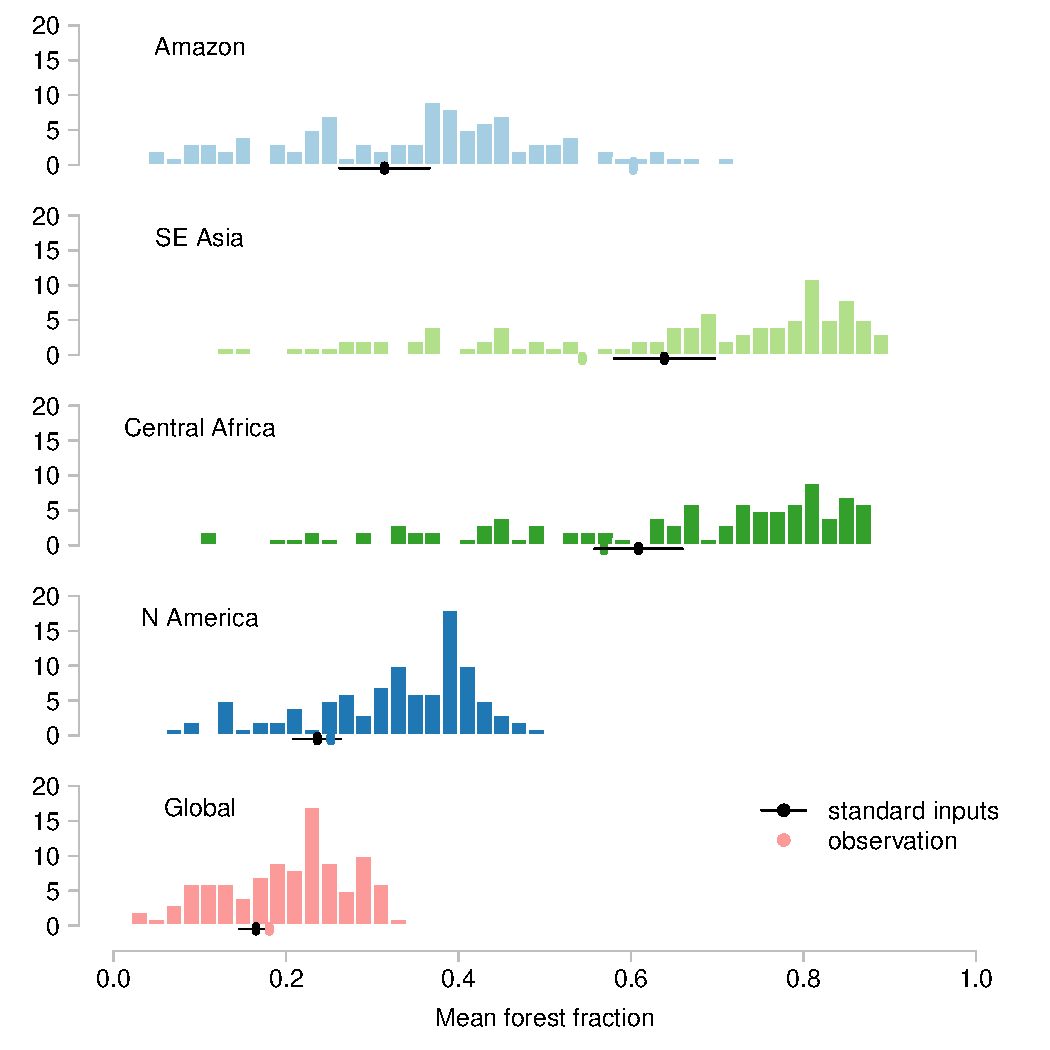
\includegraphics[width=12cm]{graphics/fraction_histogram_with_discrepancy_standard.pdf}
\caption{TEXT}
\label{fig:fraction_histogram_with_discrepancy_standard}
\end{figure}

\begin{figure}[t]
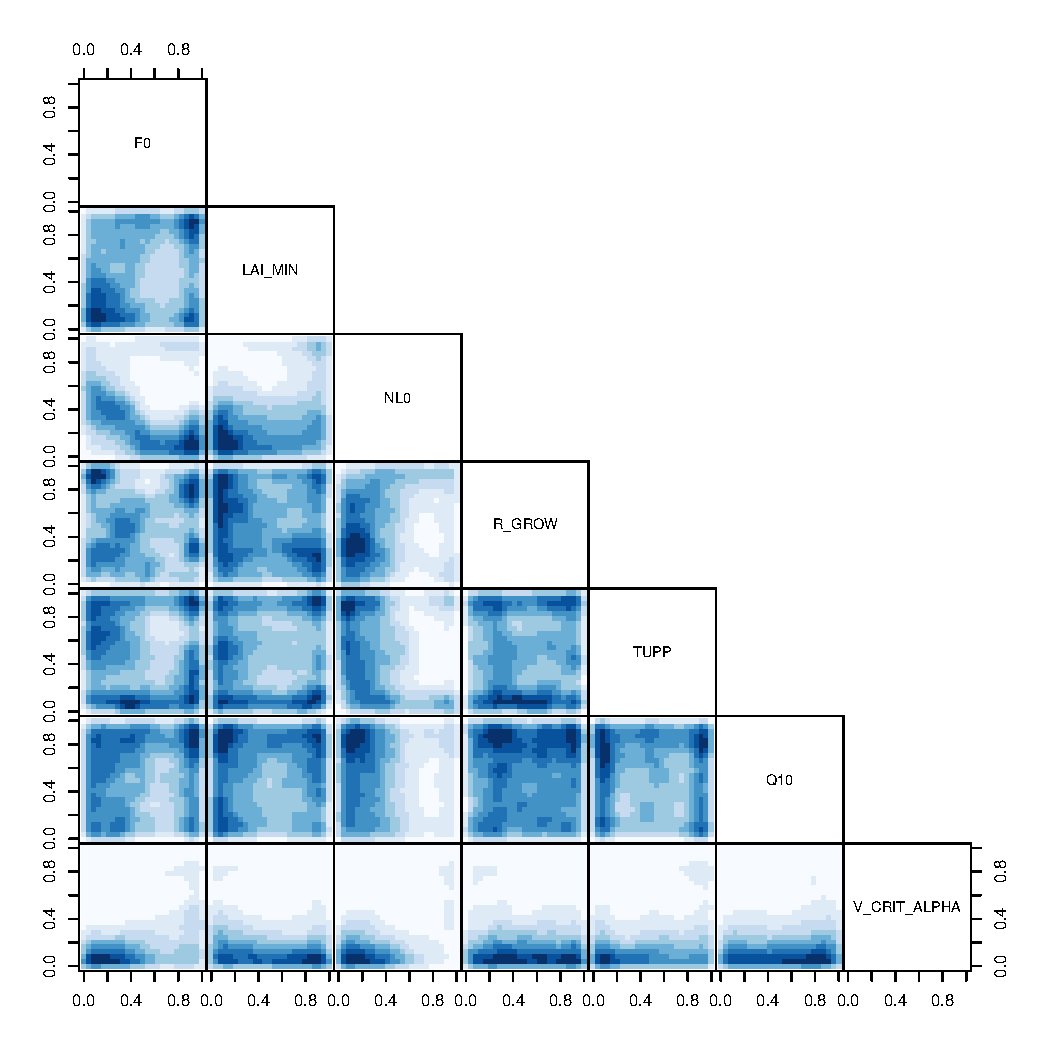
\includegraphics[width=12cm]{graphics/credible_NROY.pdf}
\caption{TEXT}
\label{fig:credible_NROY}
\end{figure}

\begin{figure}[t]
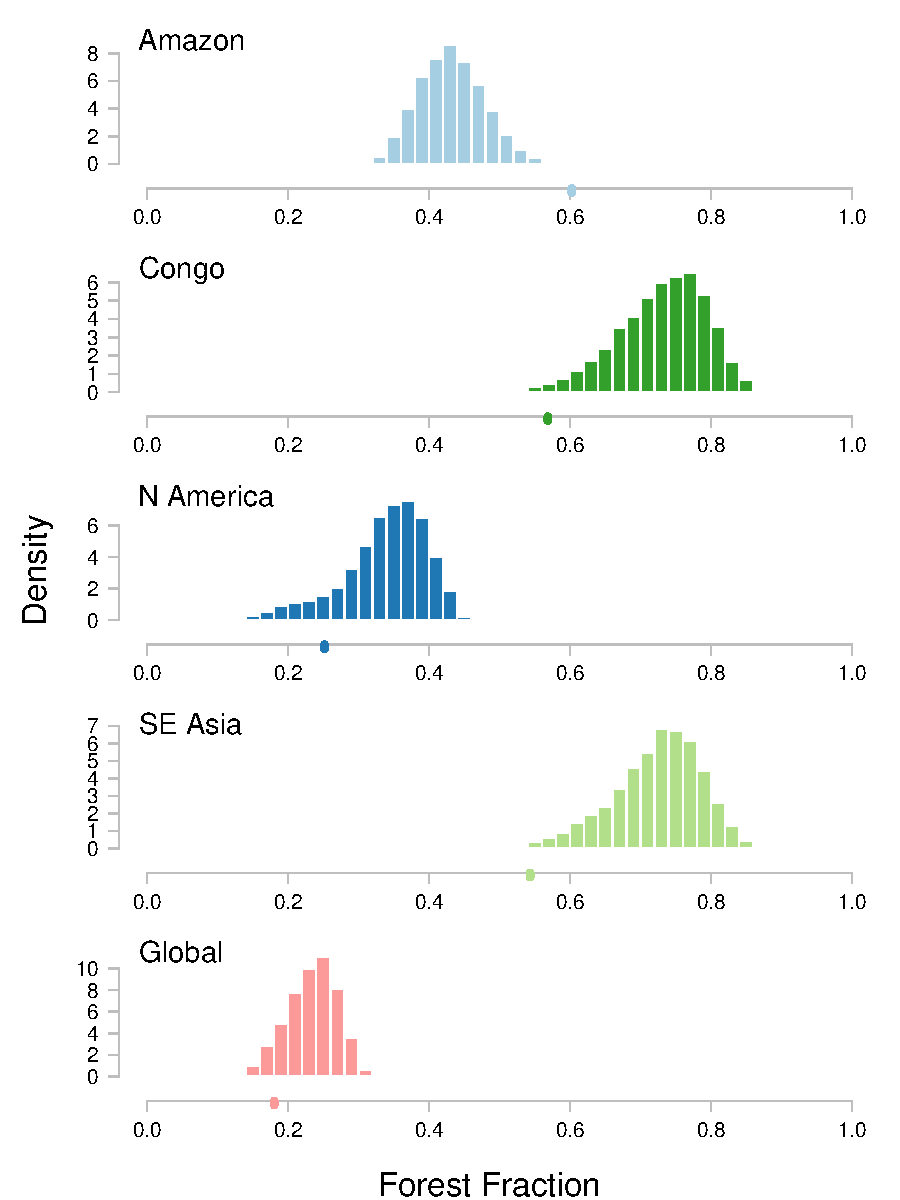
\includegraphics[width=12cm]{graphics/credible_NROY_hists.pdf}
\caption{TEXT}
\label{fig:credible_NROY_hists}
\end{figure}

\begin{figure}[t]
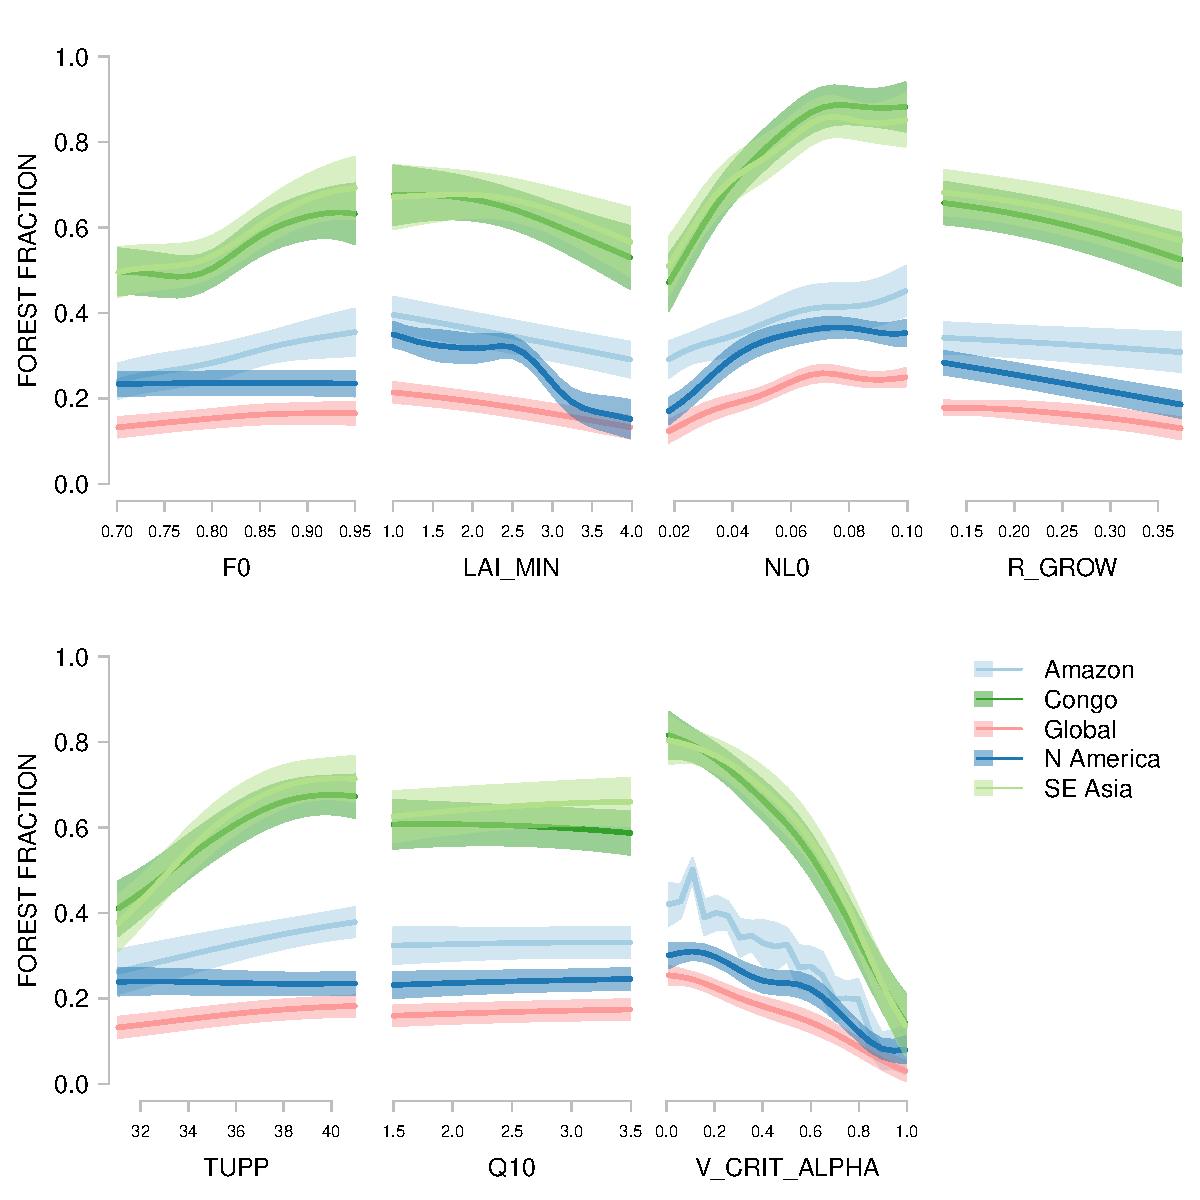
\includegraphics[width=12cm]{graphics/amaz_oat_sens.pdf}
\caption{TEXT}
\label{fig:amaz_oat_sens}
\end{figure}

\begin{figure}[t]
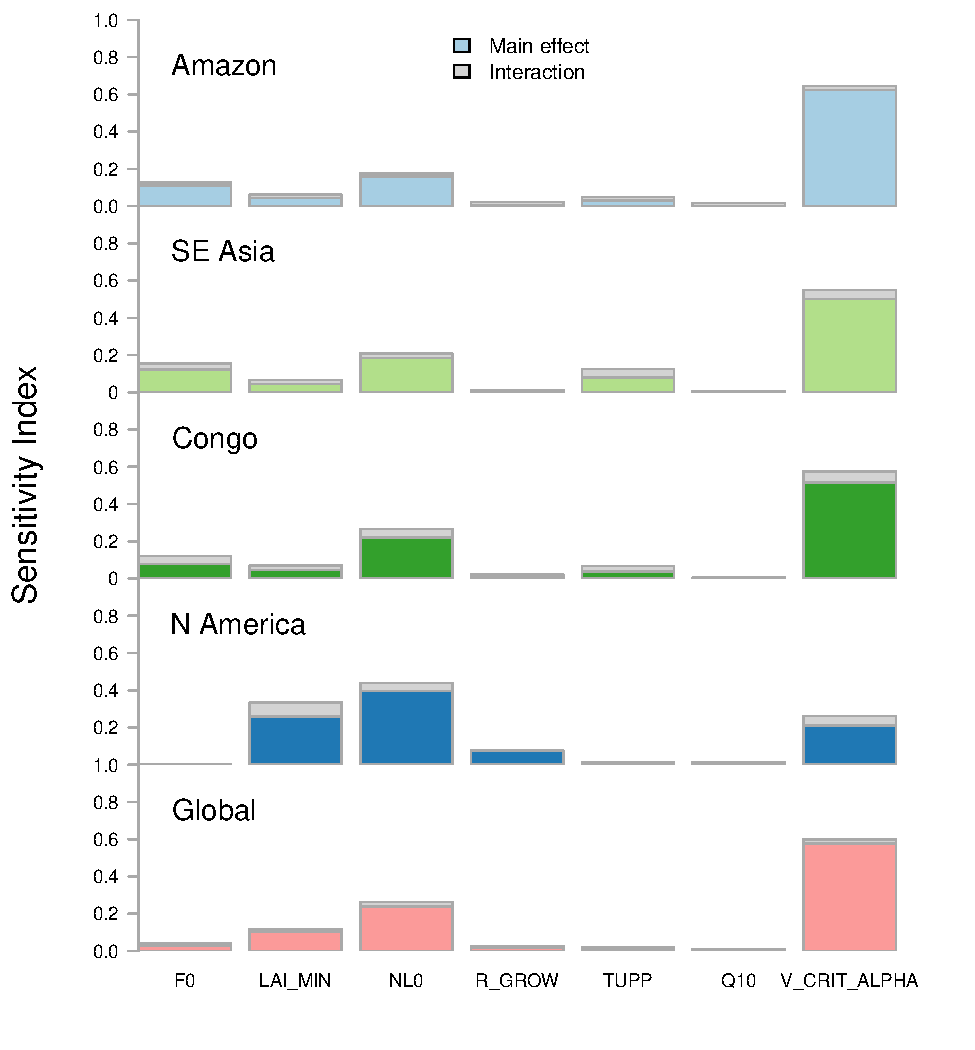
\includegraphics[width=12cm]{graphics/FAST_histograms.pdf}
\caption{TEXT}
\label{fig:FAST_histograms}
\end{figure}

\begin{figure}[t]
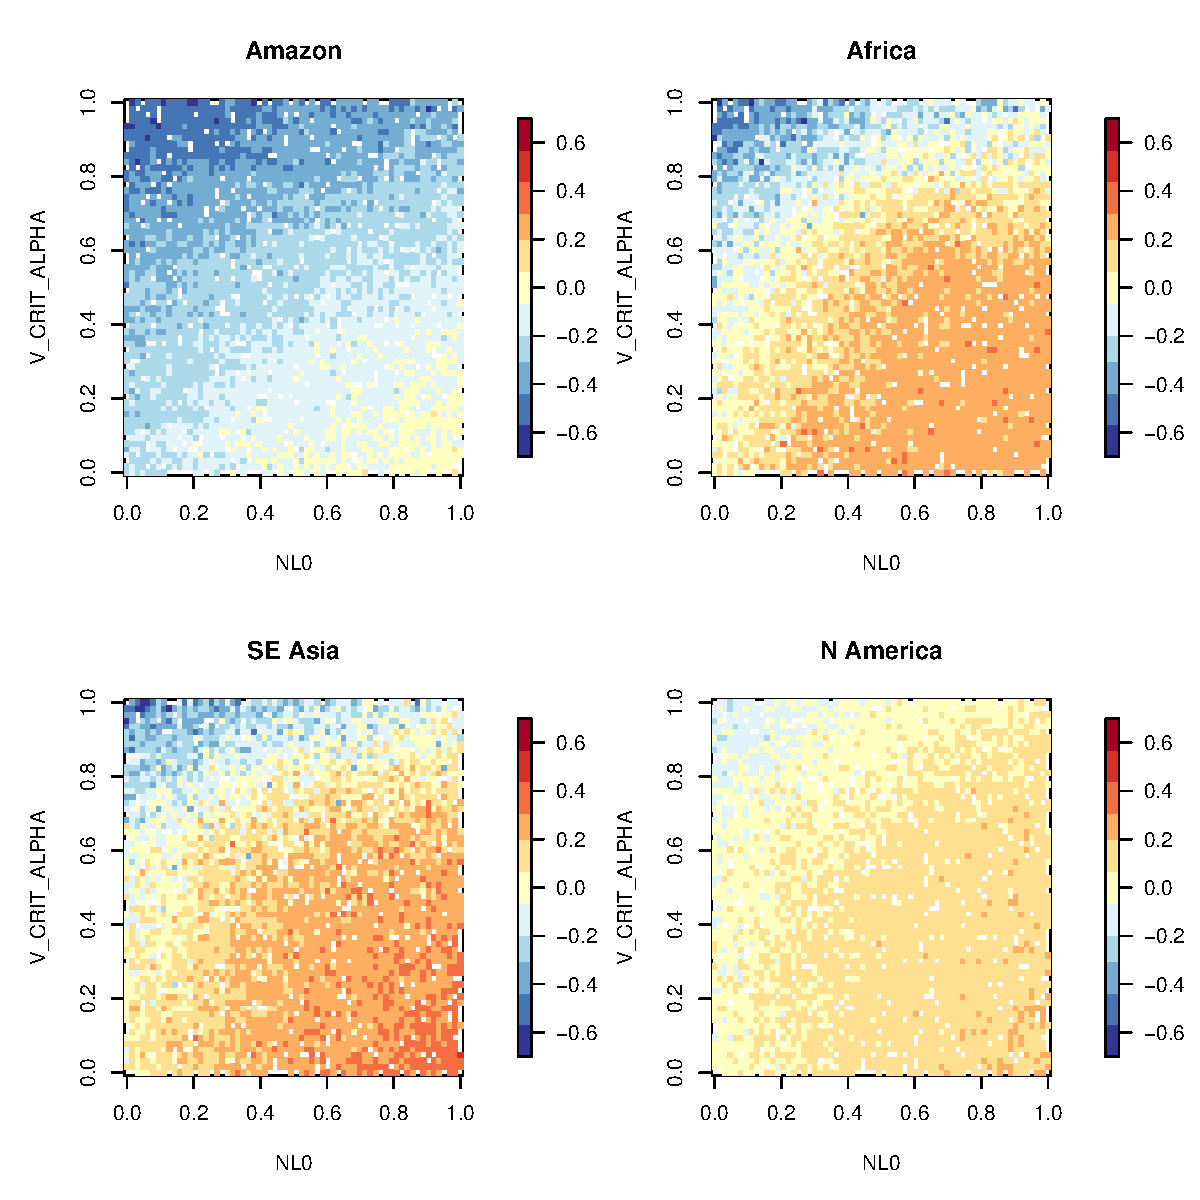
\includegraphics[width=12cm]{graphics/discrepancy_parameter_space.pdf}
\caption{TEXT}
\label{fig:discrepancy_parameter_space}
\end{figure}

\begin{figure}[t]
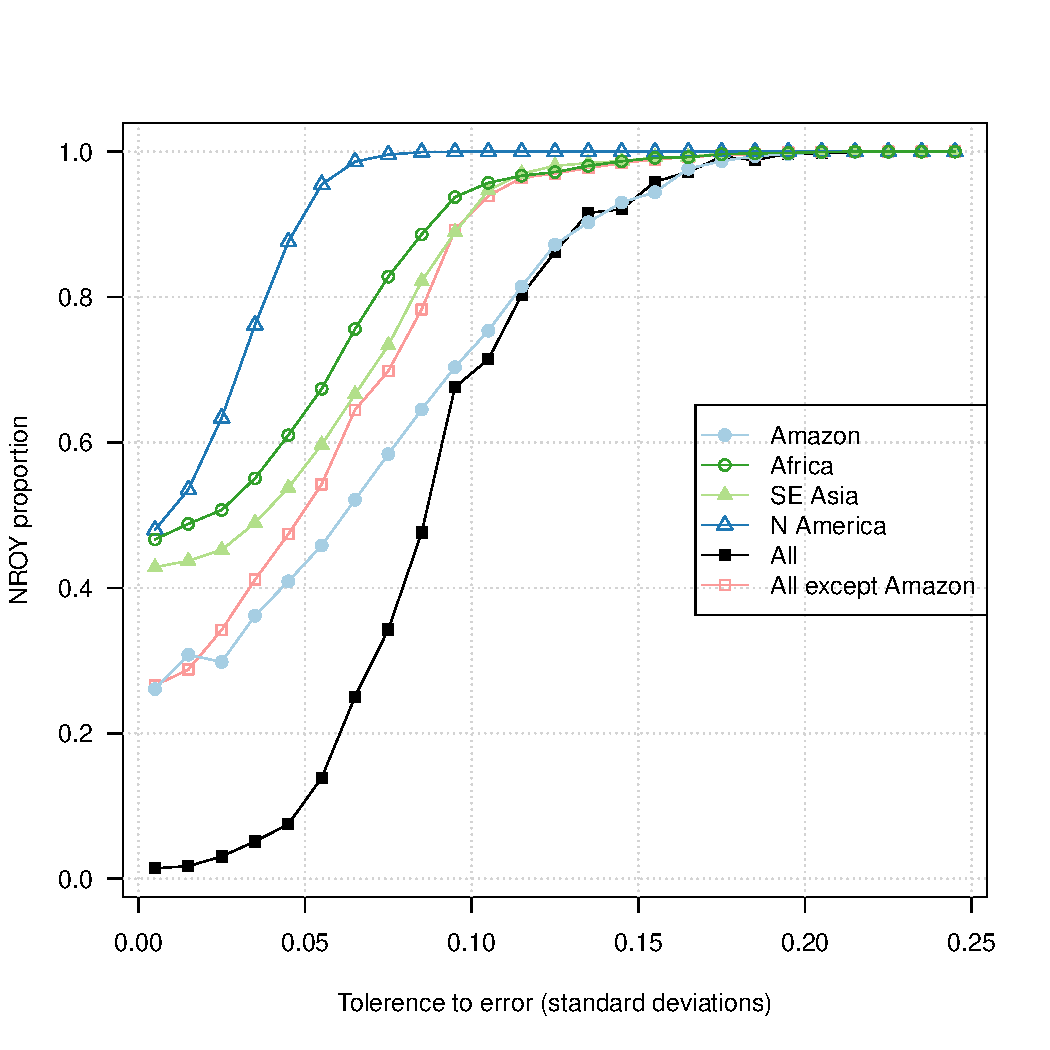
\includegraphics[width=12cm]{graphics/Prop_NROY_tolerance_unc.pdf}
\caption{TEXT}
\label{fig:Prop_NROY_tolerance_unc}
\end{figure}

\begin{figure}[t]
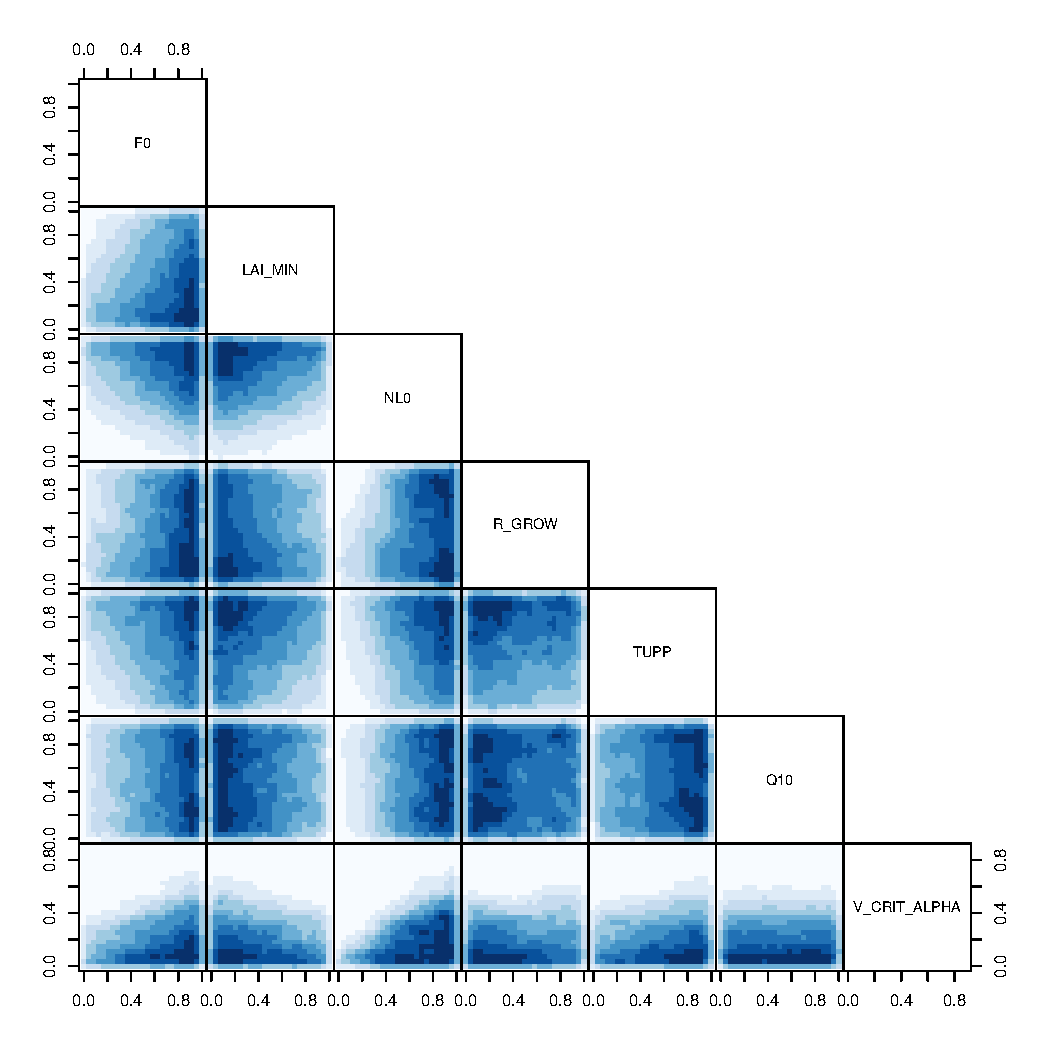
\includegraphics[width=12cm]{graphics/best_inputs_amazon.pdf}
\caption{TEXT}
\label{fig:best_inputs_amazon}
\end{figure}

\begin{figure}[t]
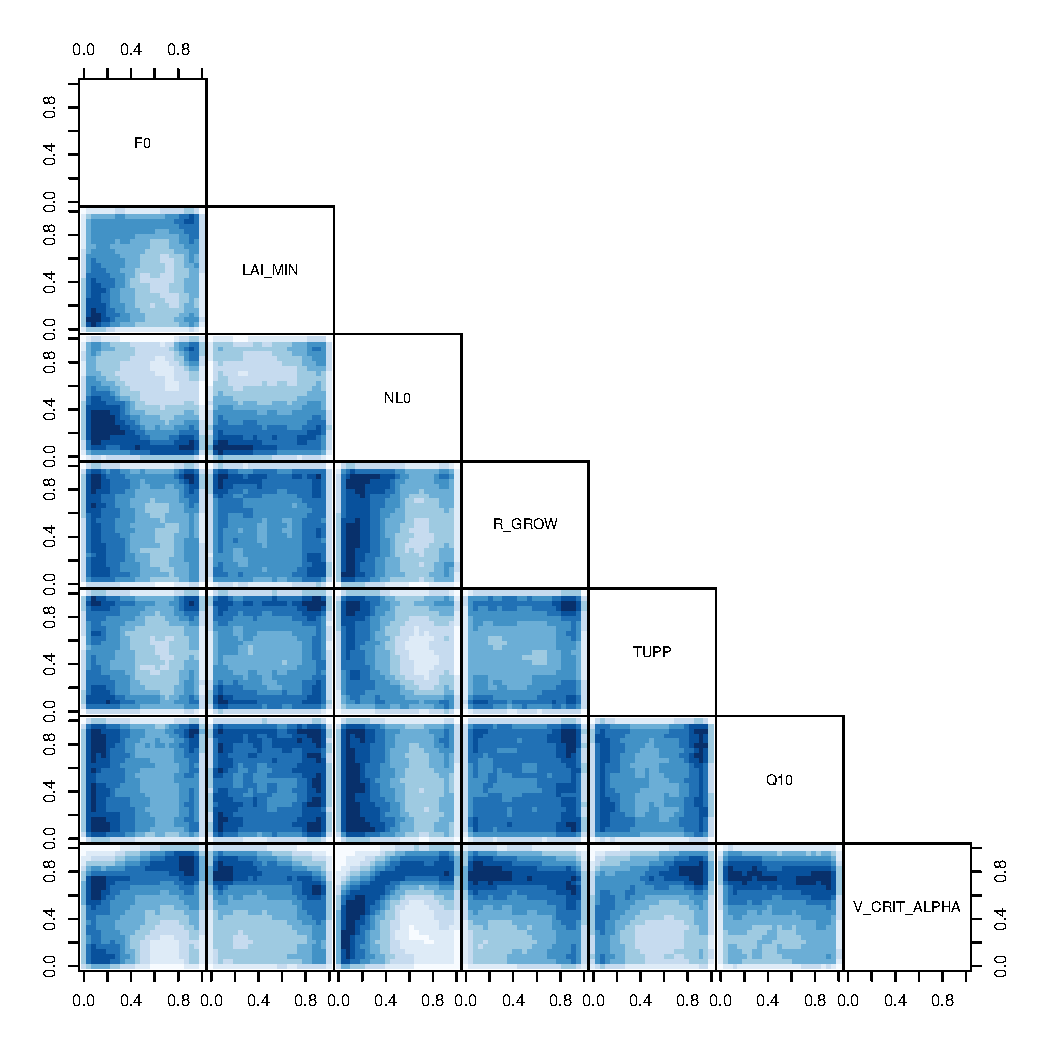
\includegraphics[width=12cm]{graphics/best_inputs_congo.pdf}
\caption{TEXT}
\label{fig:}
\end{figure}

\begin{figure}[t]
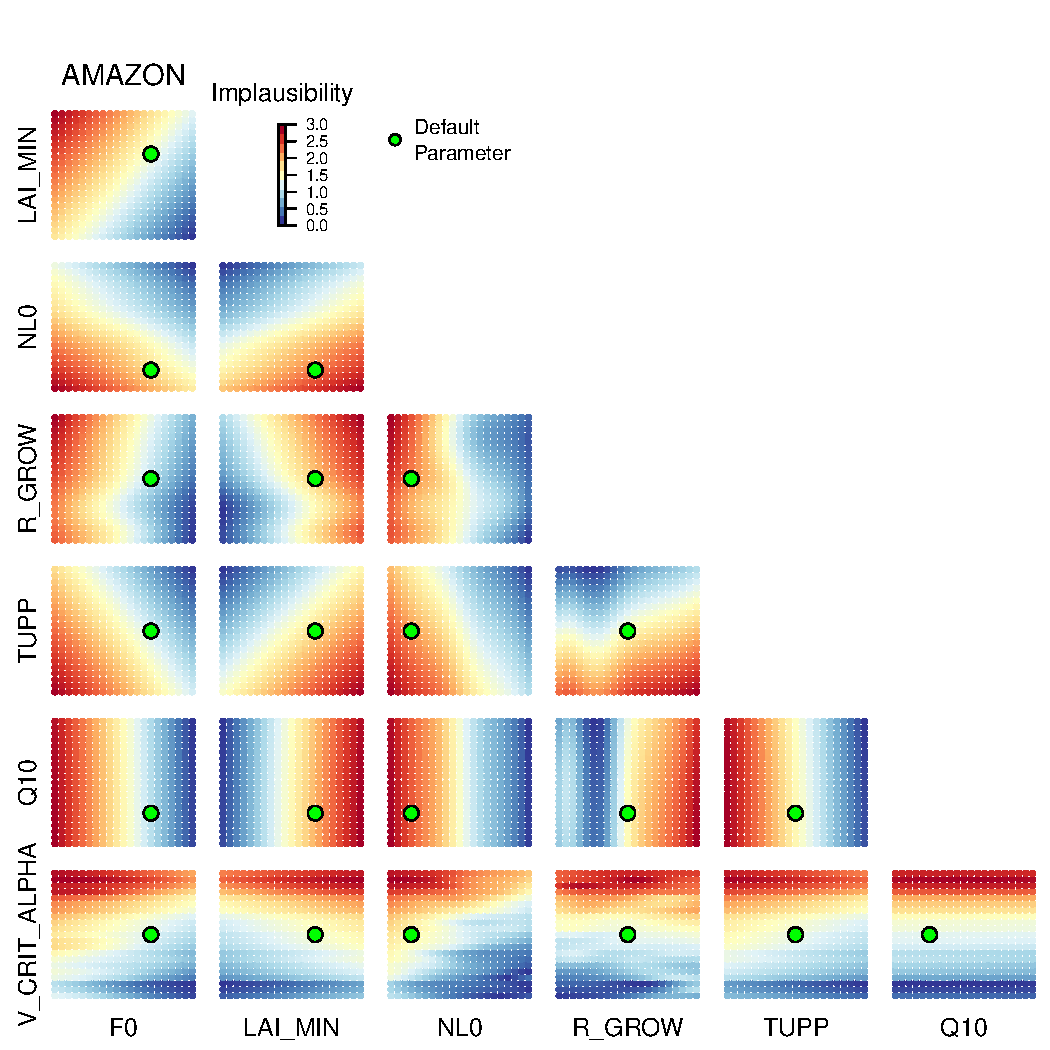
\includegraphics[width=12cm]{graphics/taat_amaz.pdf}
\caption{TEXT}
\label{fig:taat_amaz}
\end{figure}

\begin{figure}[t]
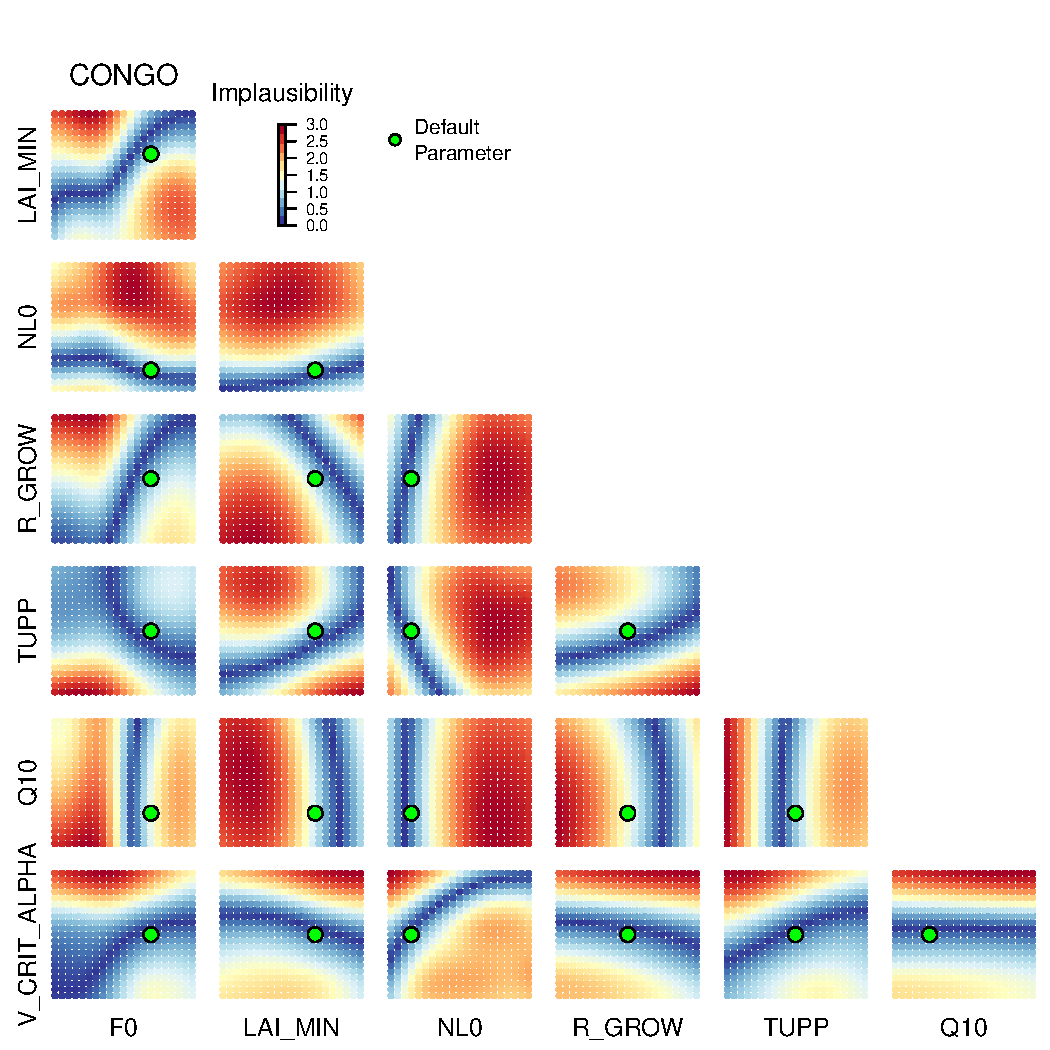
\includegraphics[width=12cm]{graphics/taat_congo.pdf}
\caption{TEXT}
\label{fig:}
\end{figure}

\begin{figure}[t]
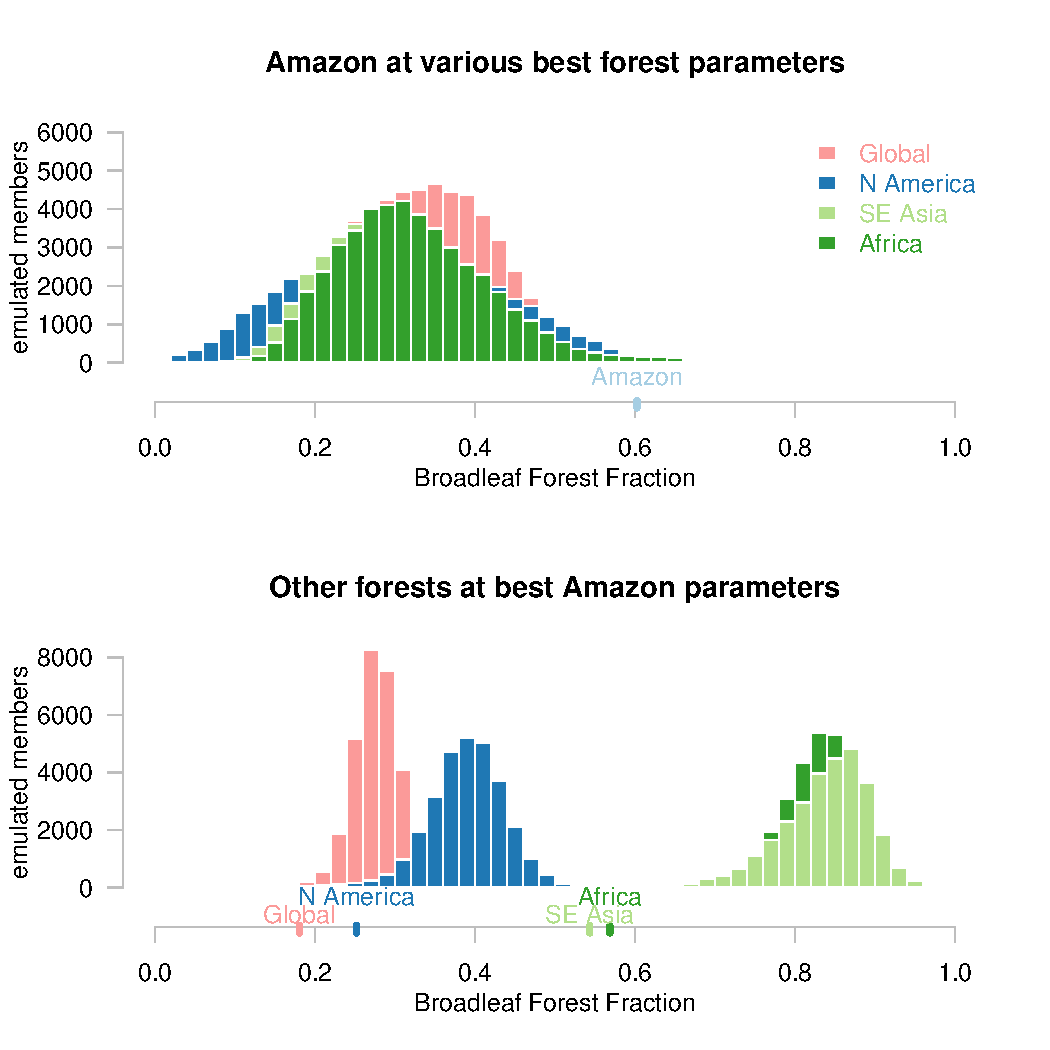
\includegraphics[width=12cm]{graphics/best_inputs_swaps_hists_Paired.pdf}
\caption{TEXT}
\label{fig:best_inputs_swaps_hists_Paired}
\end{figure}

\begin{figure}[t]
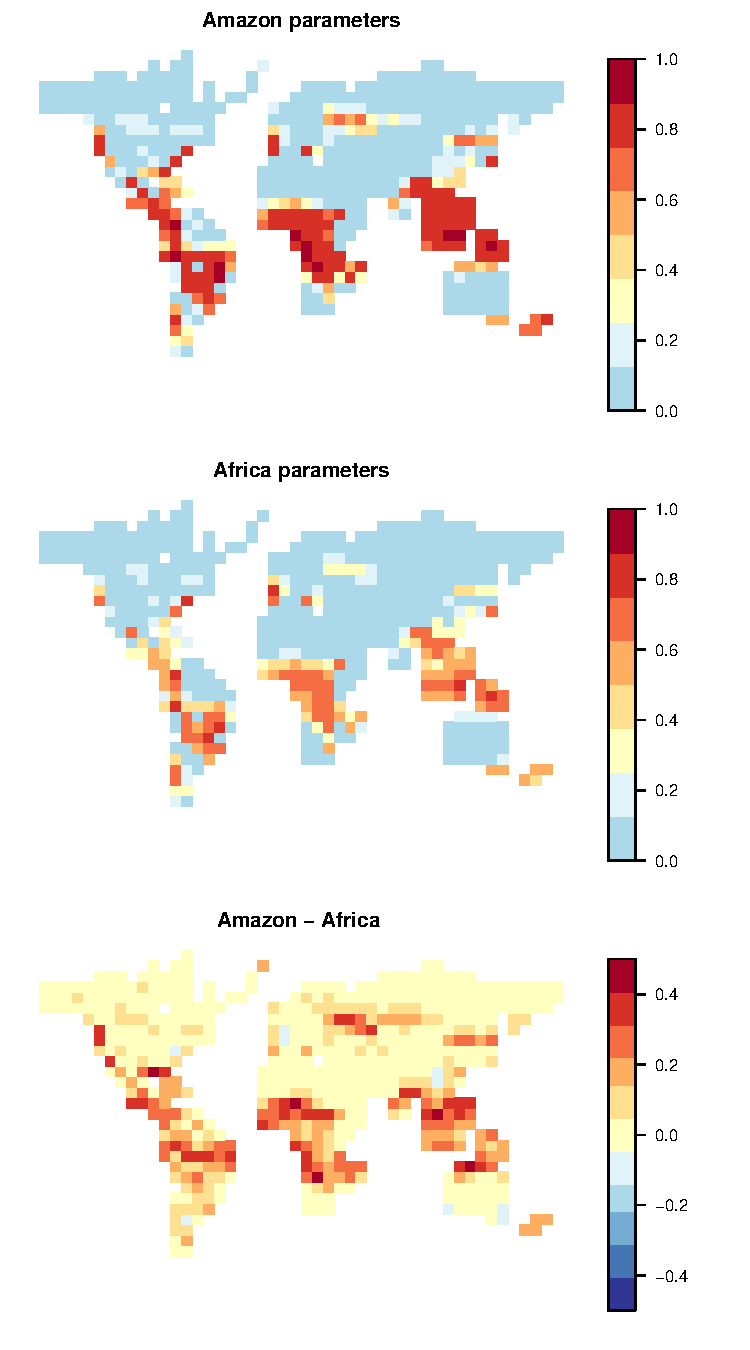
\includegraphics[width=8.3cm]{graphics/best_X_maps.pdf}
\caption{TEXT}
\label{fig:best_X_maps}
\end{figure}

\begin{figure}[t]
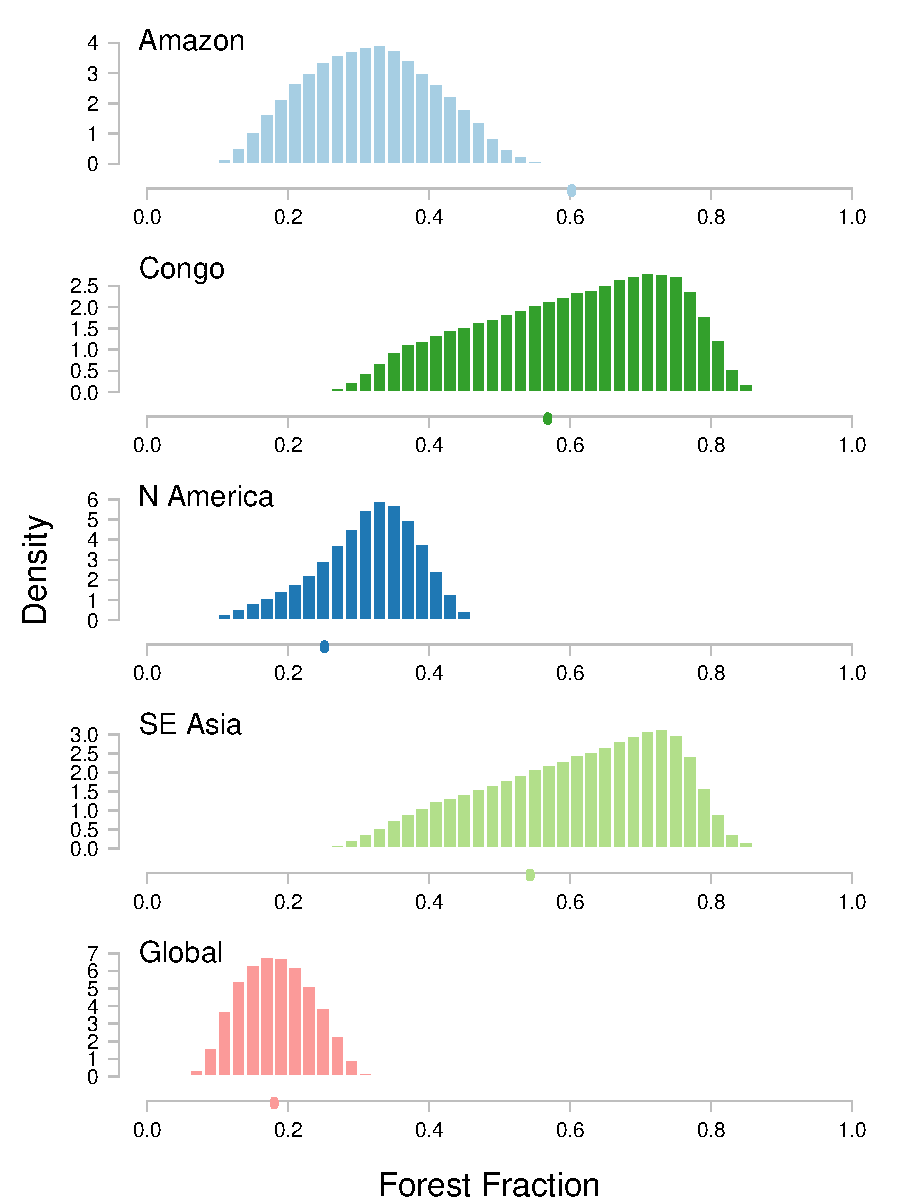
\includegraphics[width=12cm]{graphics/credible_NROY_hists_disc.pdf}
\caption{TEXT}
\label{fig:credible_NROY_hists_disc}
\end{figure}

\begin{figure}[t]
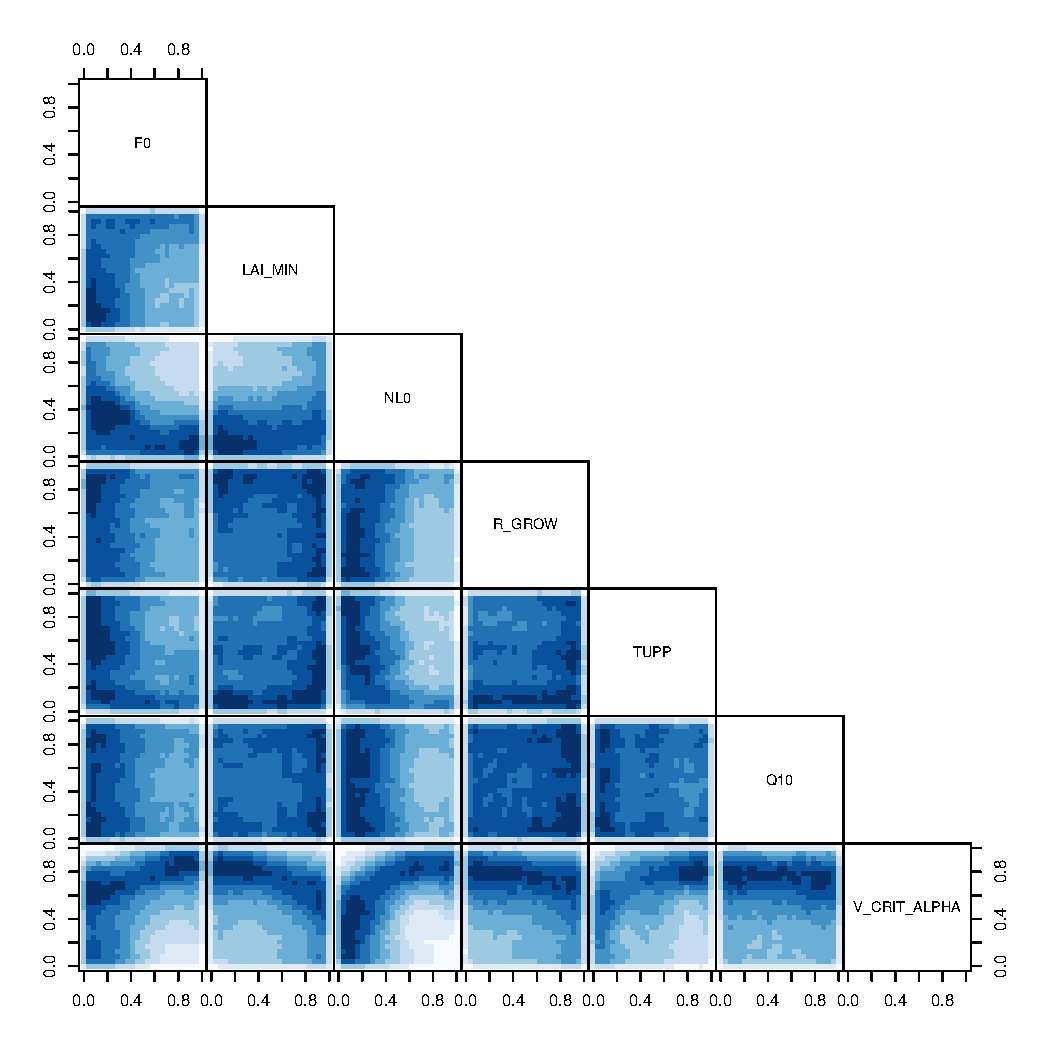
\includegraphics[width=12cm]{graphics/plausible_disc_input_space.pdf}
\caption{TEXT}
\label{fig:plausible_disc_input_space}
\end{figure}

\begin{figure}[t]
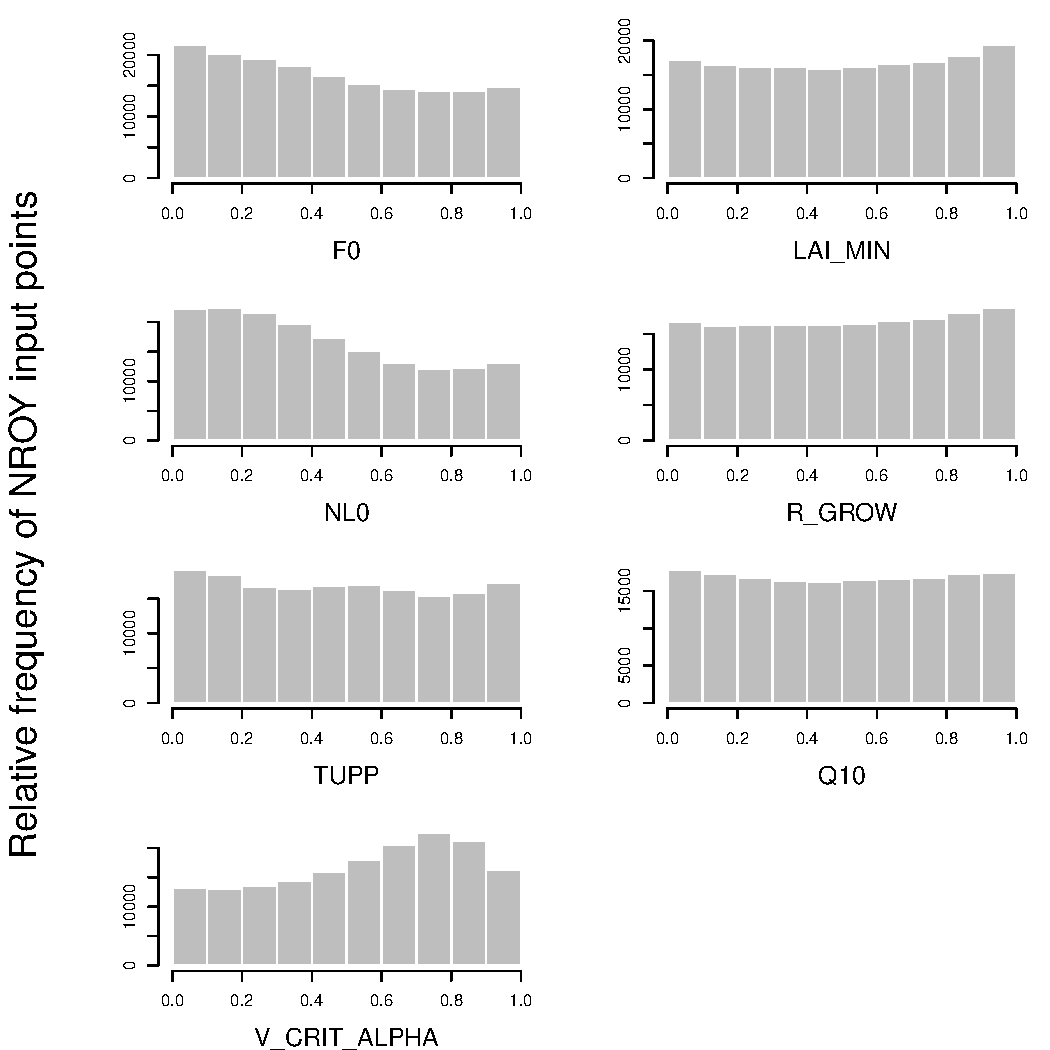
\includegraphics[width=12cm]{graphics/input_frequency_marginal.pdf}
\caption{TEXT}
\label{fig:input_frequency_marginal}
\end{figure}

%\begin{figure}[t]
%\includegraphics[width=12cm]{graphics/.pdf}
%\caption{TEXT}
%\label{fig:}
%\end{figure}



%% ONE-COLUMN FIGURES

%%f
%\begin{figure}[t]
%\includegraphics[width=8.3cm]{FILE NAME}
%\caption{TEXT}
%\end{figure}
%
%%% TWO-COLUMN FIGURES
%
%%f
%\begin{figure*}[t]
%\includegraphics[width=12cm]{FILE NAME}
%\caption{TEXT}
%\end{figure*}
%
%
%%% TABLES
%%%
%%% The different columns must be seperated with a & command and should
%%% end with \\ to identify the column brake.
%
%%% ONE-COLUMN TABLE
%
%%t
%\begin{table}[t]
%\caption{TEXT}
%\begin{tabular}{column = lcr}
%\tophline
%
%\middlehline
%
%\bottomhline
%\end{tabular}
%\belowtable{} % Table Footnotes
%\end{table}
%
%%% TWO-COLUMN TABLE
%
%%t
%\begin{table*}[t]
%\caption{TEXT}
%\begin{tabular}{column = lcr}
%\tophline
%
%\middlehline
%
%\bottomhline
%\end{tabular}
%\belowtable{} % Table Footnotes
%\end{table*}
%
%
%%% NUMBERING OF FIGURES AND TABLES
%%%
%%% If figures and tables must be numbered 1a, 1b, etc. the following command
%%% should be inserted before the begin{} command.
%
%\addtocounter{figure}{-1}\renewcommand{\thefigure}{\arabic{figure}a}
%
%
%%% MATHEMATICAL EXPRESSIONS
%
%%% All papers typeset by Copernicus Publications follow the math typesetting regulations
%%% given by the IUPAC Green Book (IUPAC: Quantities, Units and Symbols in Physical Chemistry,
%%% 2nd Edn., Blackwell Science, available at: http://old.iupac.org/publications/books/gbook/green_book_2ed.pdf, 1993).
%%%
%%% Physical quantities/variables are typeset in italic font (t for time, T for Temperature)
%%% Indices which are not defined are typeset in italic font (x, y, z, a, b, c)
%%% Items/objects which are defined are typeset in roman font (Car A, Car B)
%%% Descriptions/specifications which are defined by itself are typeset in roman font (abs, rel, ref, tot, net, ice)
%%% Abbreviations from 2 letters are typeset in roman font (RH, LAI)
%%% Vectors are identified in bold italic font using \vec{x}
%%% Matrices are identified in bold roman font
%%% Multiplication signs are typeset using the LaTeX commands \times (for vector products, grids, and exponential notations) or \cdot
%%% The character * should not be applied as mutliplication sign
%
%
%%% EQUATIONS
%
%%% Single-row equation
%
%\begin{equation}
%
%\end{equation}
%
%%% Multiline equation
%
%\begin{align}
%& 3 + 5 = 8\\
%& 3 + 5 = 8\\
%& 3 + 5 = 8
%\end{align}
%
%
%%% MATRICES
%
%\begin{matrix}
%x & y & z\\
%x & y & z\\
%x & y & z\\
%\end{matrix}
%
%
%%% ALGORITHM
%
%\begin{algorithm}
%\caption{�}
%\label{a1}
%\begin{algorithmic}
%�
%\end{algorithmic}
%\end{algorithm}
%
%
%%% CHEMICAL FORMULAS AND REACTIONS
%
%%% For formulas embedded in the text, please use \chem{}
%
%%% The reaction environment creates labels including the letter R, i.e. (R1), (R2), etc.
%
%\begin{reaction}
%%% \rightarrow should be used for normal (one-way) chemical reactions
%%% \rightleftharpoons should be used for equilibria
%%% \leftrightarrow should be used for resonance structures
%\end{reaction}
%
%
%%% PHYSICAL UNITS
%%%
%%% Please use \unit{} and apply the exponential notation


\end{document}
